\chapter{Related Work}

TODO: Introduction for this section. 

\section{Reducing the burden of self tracking}
Self tracking can solve the problem of memory recall bias, by letting the user register observation in the moment (or very close to) they occur. But requiring the user to log observation introduces a burden of the work involved in doing so. As mention traditionally this has been done with pen and paper, but with the invention of smartphones and smartwatches this burden can be reduces. The work of Ponnada et al., 2017\cite{compare} investigate the interruption burden for with both smartphones and smartwatches when used to with both regular EMA and $\mu$EMA. The difference between EMA and $\mu$EMA is that EMA will prompt the use less than $\mu$EMA, but requires the user to answer several questions back to back, where $\mu$EMA will instead prompt the user much more frequently, but only require the user to answer one question, which can be answered on the same screen showing the question. 

In a prior 4 week pilot study Ponnada et al. found that smartwatch $\mu$EMA demonstrated higher response rates and participants reported a lower perceived burden than smartphone EMA, even though the interruption rate for smartwatch $\mu$EMA was 8 times higher than smartphone EMA. In a new 4 week study they gathered data based on a smartwatch EMA in order to determine if the previous result where due to the fact that the data was gathered on a watch, or if it in fact was due to the $\mu$EMA. Their results showed that there were no statistically significant differences in compliance, completion, and first-prompt response rates observed between smartphone EMA and smartwatch EMA. But smartwatch $\mu$EMA response rates where significantly higher than smartwatch EMA. Their results suggest that the higher compliance and lower perceived burden is more likely to do with $\mu$EMA than the device itself and that compliance with EMA may not improve simply by changing the device.

The work of Ponnada et al. only looked into EMA where the device prompts the user for information, not situations where the user registers an observation. In his thesis Kami\'nski, 2016\cite{tomas} investigates how to enable self logging with different forms of input: a binary sample, selection input form a list, VAS and a numerical scale. He designed and implemented all of the input methods onto a smartwatch, where on the watch face each method input method could be selected. In figure \ref{tomas_design} we can see his design, the watch face has a shortcut for each input method. In figure \ref{tomas_design2} we see how the interaction occurs, and that it takes 1-3 touches to log the desired data depending on the input method.

\begin{figure}[h!]
    \centering
    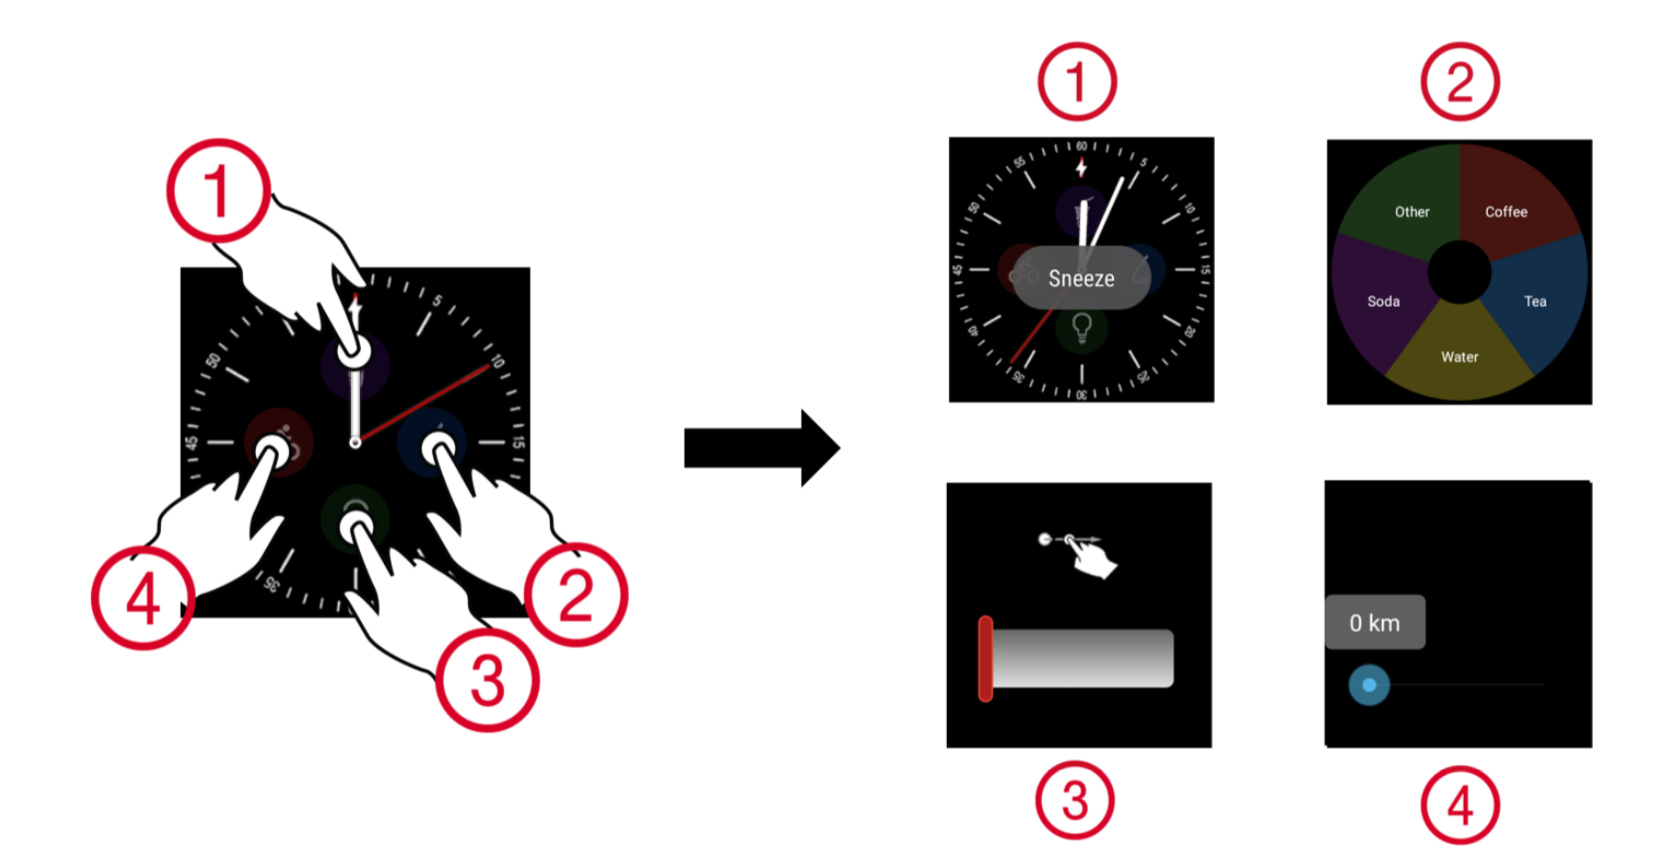
\includegraphics[width=1\textwidth]{figures/tomas_design.png}
    \caption{Design for self logging on a smartwatch by Kami\'nski\cite{tomas}}
    \label{tomas_design}
\end{figure}

\begin{figure}[h!]
    \centering
    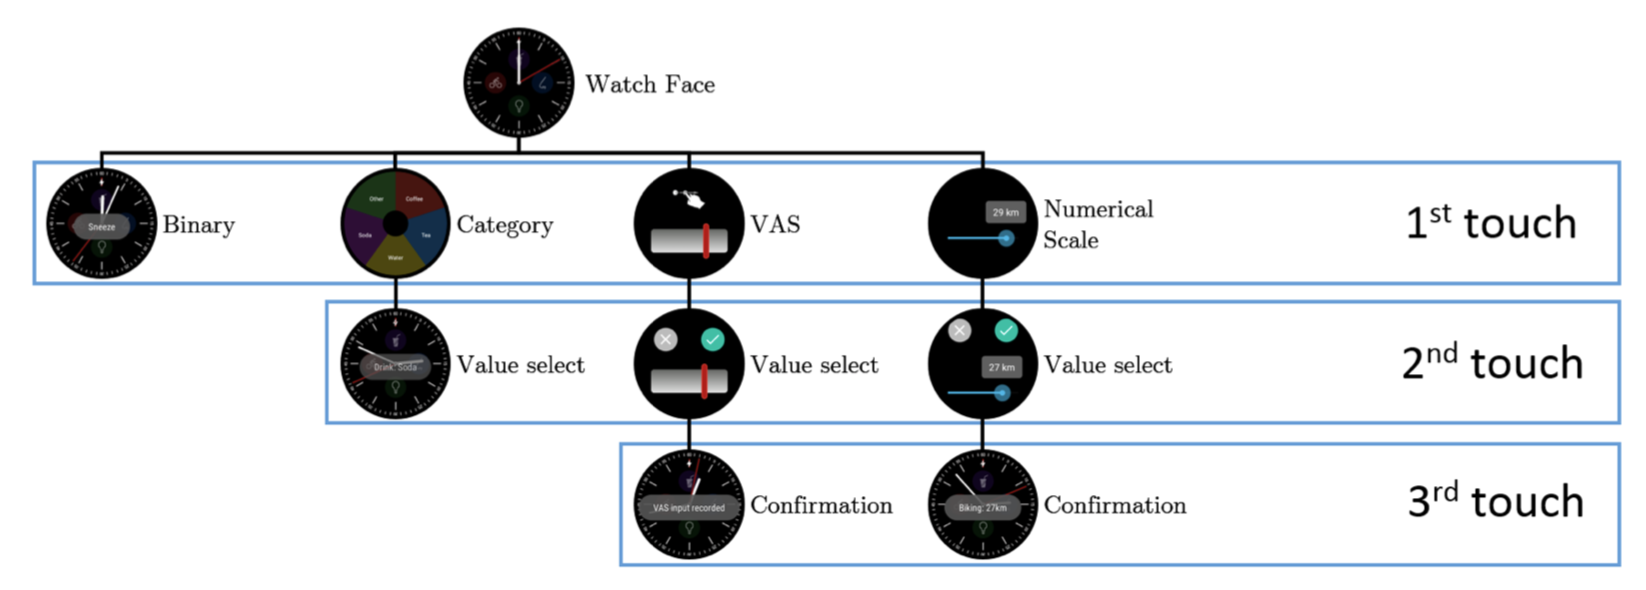
\includegraphics[width=1\textwidth]{figures/tomas_design2.png}
    \caption{Interaction for self logging on a smartwatch by Kami\'nski\cite{tomas}}
    \label{tomas_design2}
\end{figure}

For comparison Kami\'nski also implemented his a similar design on a smartphone following the \emph{Android material design guide}\cite{android_design} and conducted an experiment where he compared the two devices performance (interaction time, lower is better). His result showed a reduction in the user interaction time by approximately 30\% on average, thus successfully reducing the burden related to self logging. 

Even though Kami\'nski design was a success, there persist an underlying problem with smartwatches; that they still require the user to user to activate them (often by tapping the screen or rotating their arm) and then the user has to look at the screen to touch the right section to register the input. Dam-Jensen, 2018\cite{dam} investigates this issue in his thesis. He introduces three ways of performing self logging, all using a \say{smartbutton} (wireless button connected to smartphone/smartwatch) to achieve a display-less logging system. The three input method that Dam-Jensen designed was:

\begin{enumerate}
	\item Hold Button: Measure the time the button is held down.
	\item Rotate Lower Arm: Using the built in gyroscope in the smartbutton, the difference in rotation from when the button was pressed to it was released is measured. In order to achieve a measurement the user would hold the button in the hand, rotate the lower arm to a neutral position, hold down the button, rotate the lower arm to the end position and release the button. 
	\item Rotate Upper Arm Around Elbow: Similar to the previous method, but instead of rotating the lower arm, the user would raise/lower his/hers upper arm around the elbow.
\end{enumerate}

For a comparison baseline method a standard VAS was used. In order to compare his three methods to the VAS Dam-Jensen conducted an experiment based on the work of Matejka et al., 2016 \cite{grey}, where participants are asked to rate a color between white and black on a grey scale where the colors are equally spaced out on the CIELAB color space\cite{cielab} (more on this later). His results showed that there where no significant difference in accuracy between his three designed input methods compared and the baseline, thus meaning that all three methods are viable and could be used for self logging, and in their simple nature can reduce the burden on the user.

\section{Real world use case}

Larsen et al., 2017\cite{eg}



\section{Comparing ratings of behavior}
Matejka et al., 2016 \cite{grey}

Borg and Bord, 1991\cite{borg}